\documentclass[12pt]{article}
\bibliographystyle{IEEEtran}
\usepackage{graphicx,fancyhdr,parskip}
\setlength{\parskip}{.5cm plus4mm minus3mm}
\usepackage[margin=1in]{geometry}
\usepackage[colorlinks]{hyperref}
\usepackage{color}
\definecolor{darkblue}{rgb}{0,0,0.5}
\hypersetup{
    colorlinks=true,
    urlcolor=blue,
    citecolor=black,
    linkcolor=darkblue
}
\usepackage[nonumberlist]{glossaries}
\renewcommand{\glossarysection}[2][]{}
\makeglossaries
\usepackage{makeidx}
\makeindex
\makeatletter
  \renewcommand\@seccntformat[1]{\csname the#1\endcsname.\quad}
\makeatother
%\def\thesection {\Alph{section}}
%\def\thesubsection {\alph{subsection}}
%\def\thesubsubsection {\arabic{subsubsection}}
%\usepackage{titlesec}
%\titlespacing{\subsection}{2em}{0pt}{0pt}
%\titlespacing{\subsubsection}{4em}{0pt}{0pt}

\pagestyle{fancy}
\fancyhead[LO]{SiQuoia test plan (Team Q06)}
\fancyfoot[RO]{\copy SQ06 \year}

\hyphenation{op-tical net-works semi-conduc-tor}

\begin{document}
\title{CS160 - SiQuoia Test Plan \\ {\normalsize Version 1}}

%\author{ Ryan Alcoran \and Joe Lee \and Shivalik Narad \and Nam Phan
%  \and Swapna Vemparala \and Amber Wong }
\author{{\Large Team Q06}}

\begin{titlepage}
\maketitle

{\bf Project Team}
\begin{center}
\begin{tabular}{p{4cm} l}
{\bf Names}         & {\bf Roles} \\[.5em]
Joe Lee             & Business Manager \\[1em]
Swapna Vemparala    & Project Manager \\[1em]
Shivalik Narad      & Development Manager 1 \\[1em]
Nam Phan            & Development Manager 2 \\[1em]
Amber Wong          & Risk Manager \\[1em]
Ryan Alcoran        & Test Manager
\end{tabular}
\end{center}

{\bf Revision History}
\begin{center}
\begin{tabular}{|l|l|l|}
\hline
{\bf Date}      & {\bf Reasons for change}  & {\bf Version} \\
\hline
11/24/2013      & Initial creation          & v1 \\
\hline
\end{tabular}
\end{center}

\end{titlepage}

\tableofcontents

\newpage
\section{Introduction}

\subsection{Purpose}
This document contains the test plan for all components of the SiQuoia
system, based on the requirements voted on by the class. The test plan
defines a systematic and detailed approach for testing the
system. This document is intended for all the stakeholders of the
SiQuoia system.

\subsection{Scope}
The SiQuoia software implements an online multiple choice question
(MCQ) game. This document covers the test plan in order to ensure that
SiQuoia meets all the requirements specified by the client. This
document also covers the traceability matrix for the SiQuoia system so
that all the requirements can be traced back to the design and test
cases.

\subsection{List of definitions and abbreviations}

\subsubsection{Definitions}
\begin{center}
\begin{tabular}{p{5cm}p{12cm}}
functional requirement      & requirement that defines a specific 
                              function of SiQuoia \\[2em]
game store                  & feature of SiQuoia whereby users may 
                              purchase quiz packets and memorabilia \\[2em]
nonfunctional requirement   & requirement specifying criteria that can
                              be used to judge a function of SiQuoia
                              and that persists throughout the system \\[2em]
SeQuoia                     & SiQuoia, Inc. (industry industry leader 
                              in providing education, training and 
                              certification software for corporate 
                              training via simple quiz programs 
                              testing learning and retentivity) \\[2em]
SiQuoia                     & Simple Intelligence Quotient Increasing
                              Application \\[2em]
topic                       & specific subject of a question; a topic
                              can have multiple subtopics, which have
                              full characteristics like a topic \\[2em]
quiz                        & test with 20 questions and four answers
                              for each question, with only answer being
                              correct
\end{tabular}
\end{center}

\subsubsection{Abbreviations}
\begin{center}
\begin{tabular}{p{5cm}p{12cm}}
MVC                         & Model-View-Controller design pattern \\[2em]
MCQ                         & multiple choice question
\end{tabular}
\end{center}

\subsection{Overview}
This document is organized as follows. Section 1 is an introduction to 
the Test Plan document. Section 2 consists of the Test plan, and 
section 3 contains the Traceability matrix.

\section{Test plan}
The test plan covers how the implemented requirements will be tested, 
the expected results of running these tests, and whether the actual 
result matches the expected result.

\subsection{Test matrix}
\begin{center}
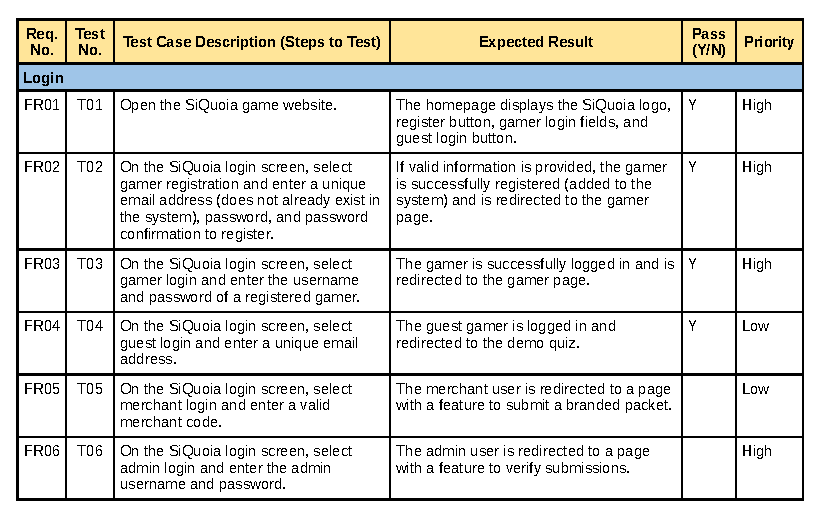
\includegraphics[width=\textwidth]{tests0}
\newpage
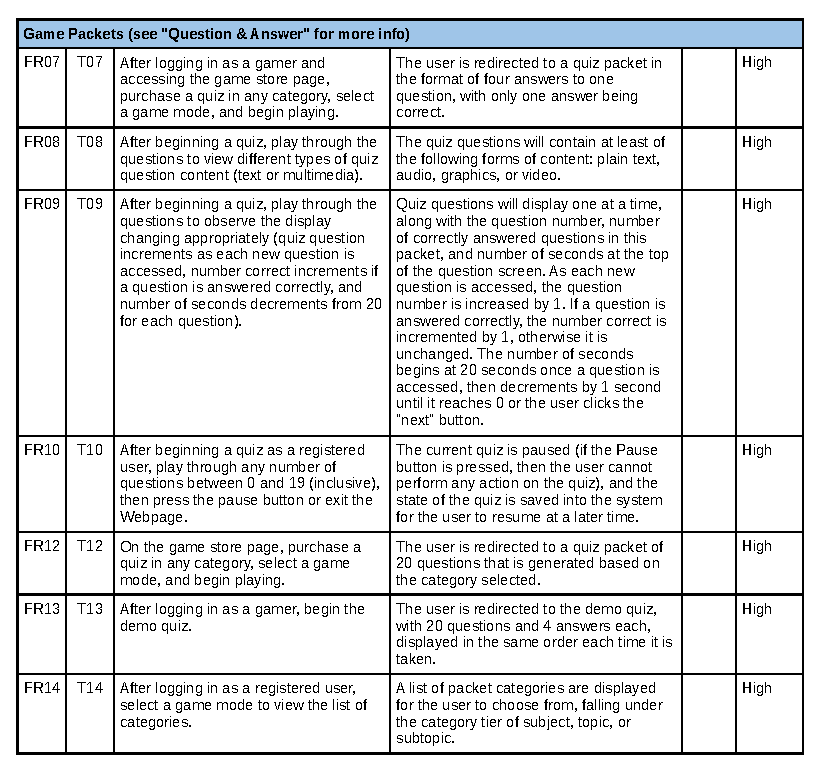
\includegraphics[width=\textwidth]{tests1}
\newpage
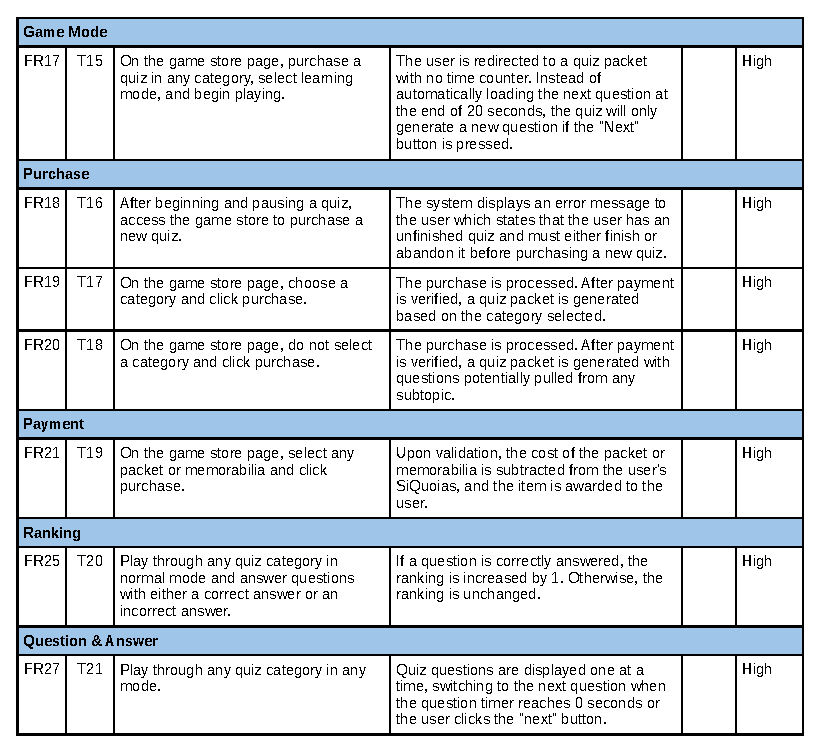
\includegraphics[width=\textwidth]{tests2}
\newpage
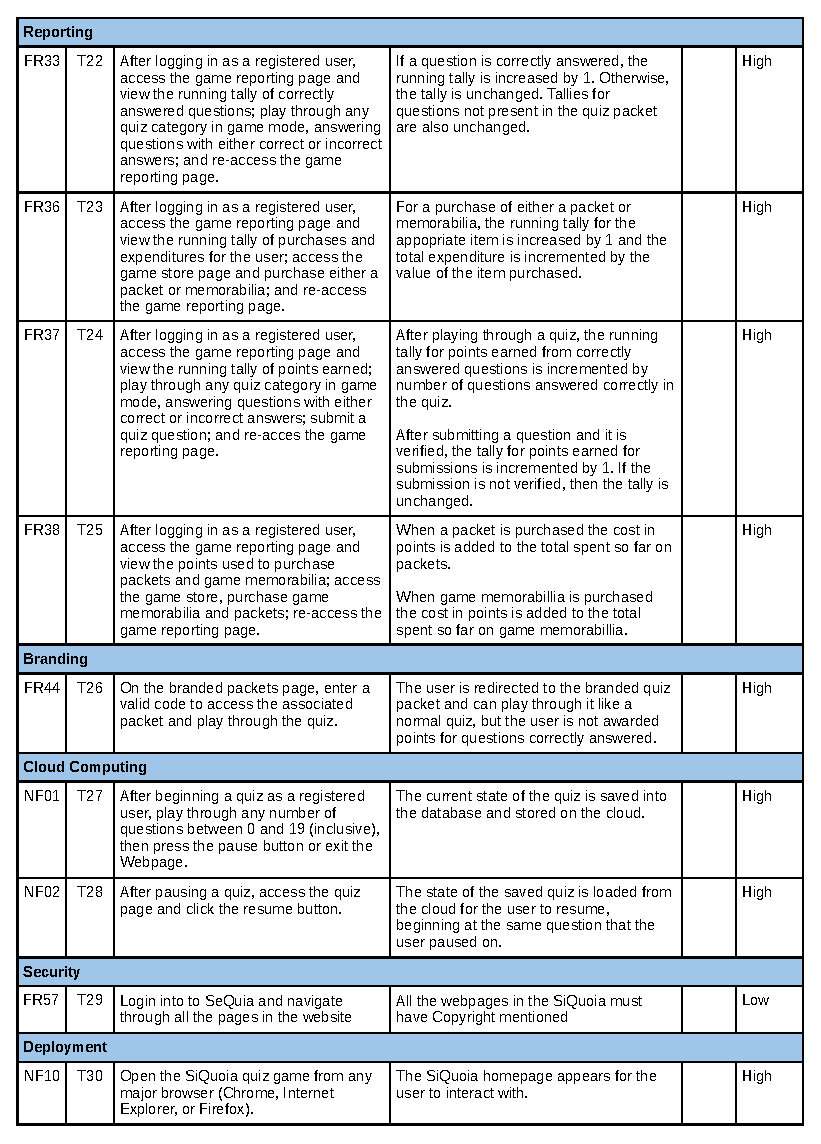
\includegraphics[width=\textwidth]{tests3}
\end{center}


\section{Requirement traceability}
The traceability matrix contains the requirement, description, type of 
requirement (E~---~essential, D~---~desirable, O~---~optional), where the 
requirement can be located throughout the design process, and whether 
it has been implemented in the code.

\subsection{Traceability matrix}
\begin{center}
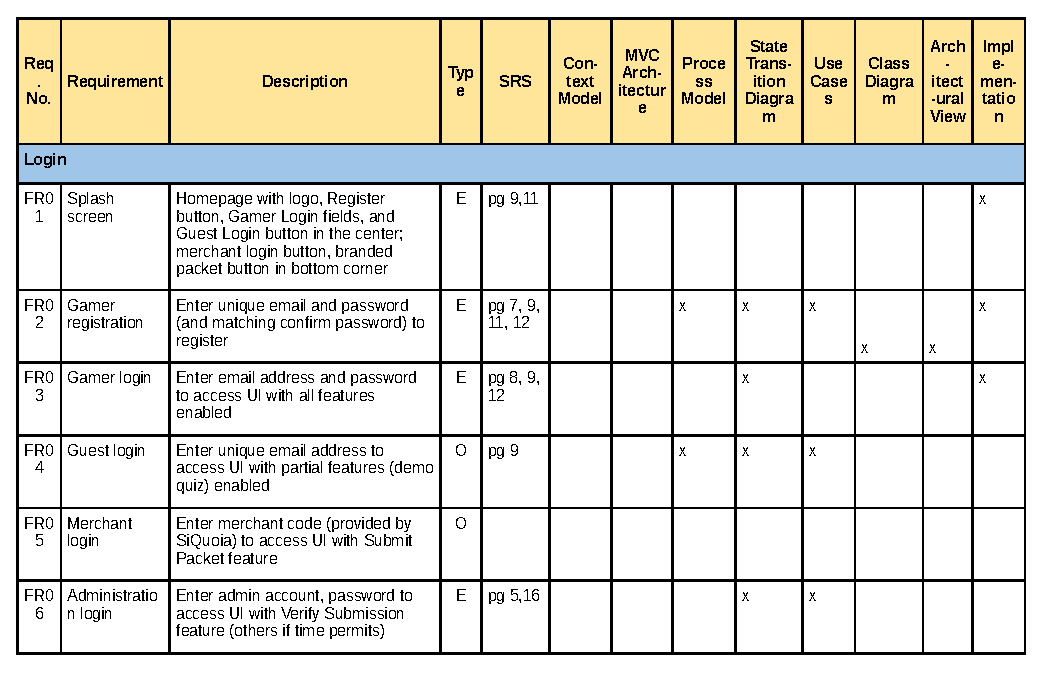
\includegraphics[width=\textwidth]{trace0}
\newpage
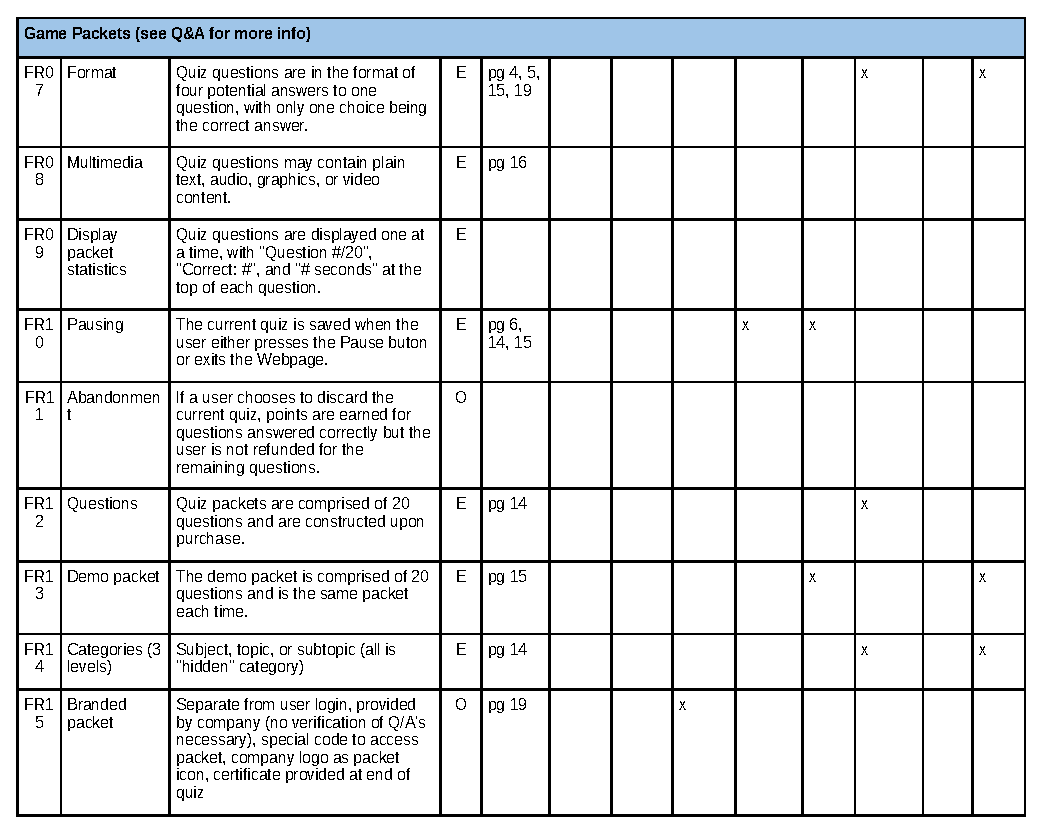
\includegraphics[width=\textwidth]{trace1}
\newpage
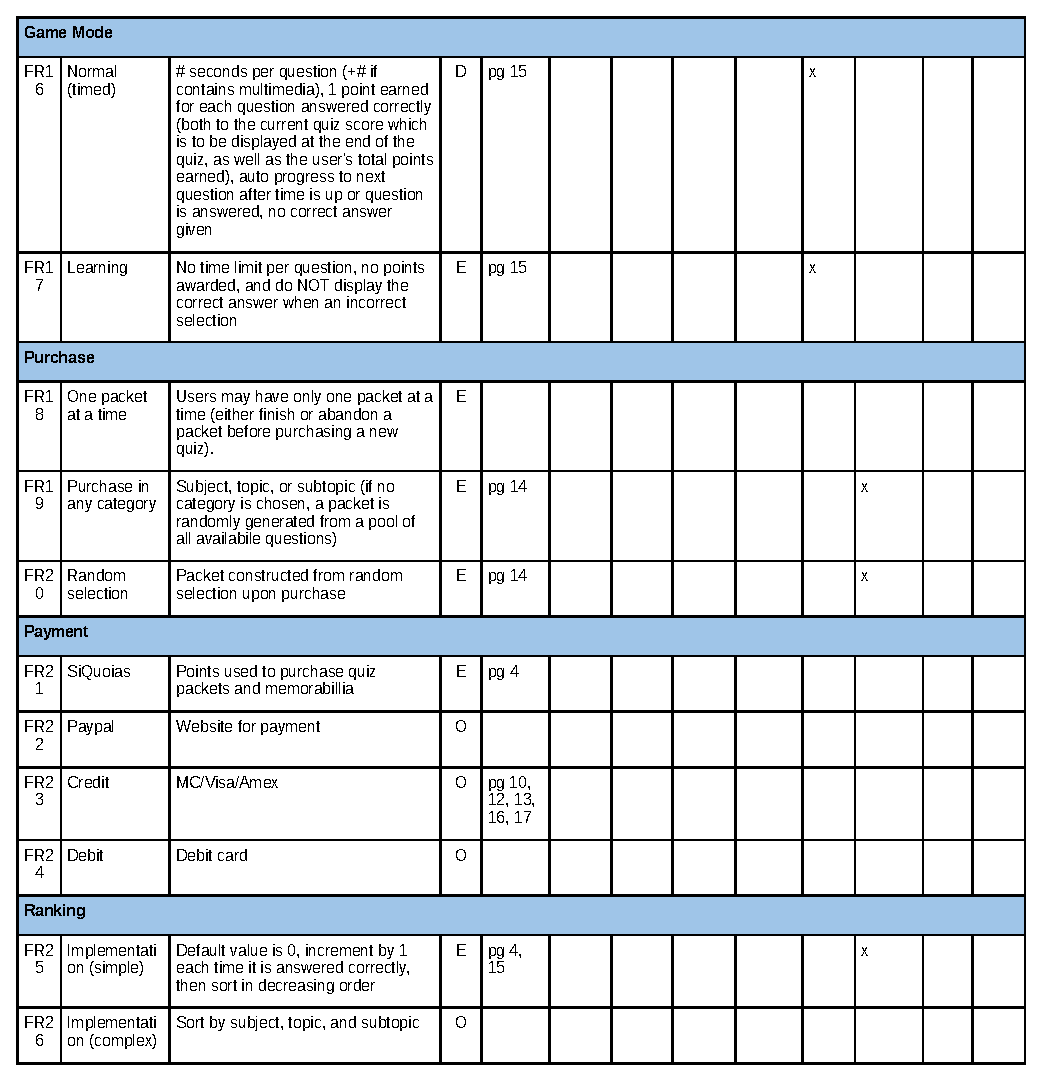
\includegraphics[width=\textwidth]{trace2}
\newpage
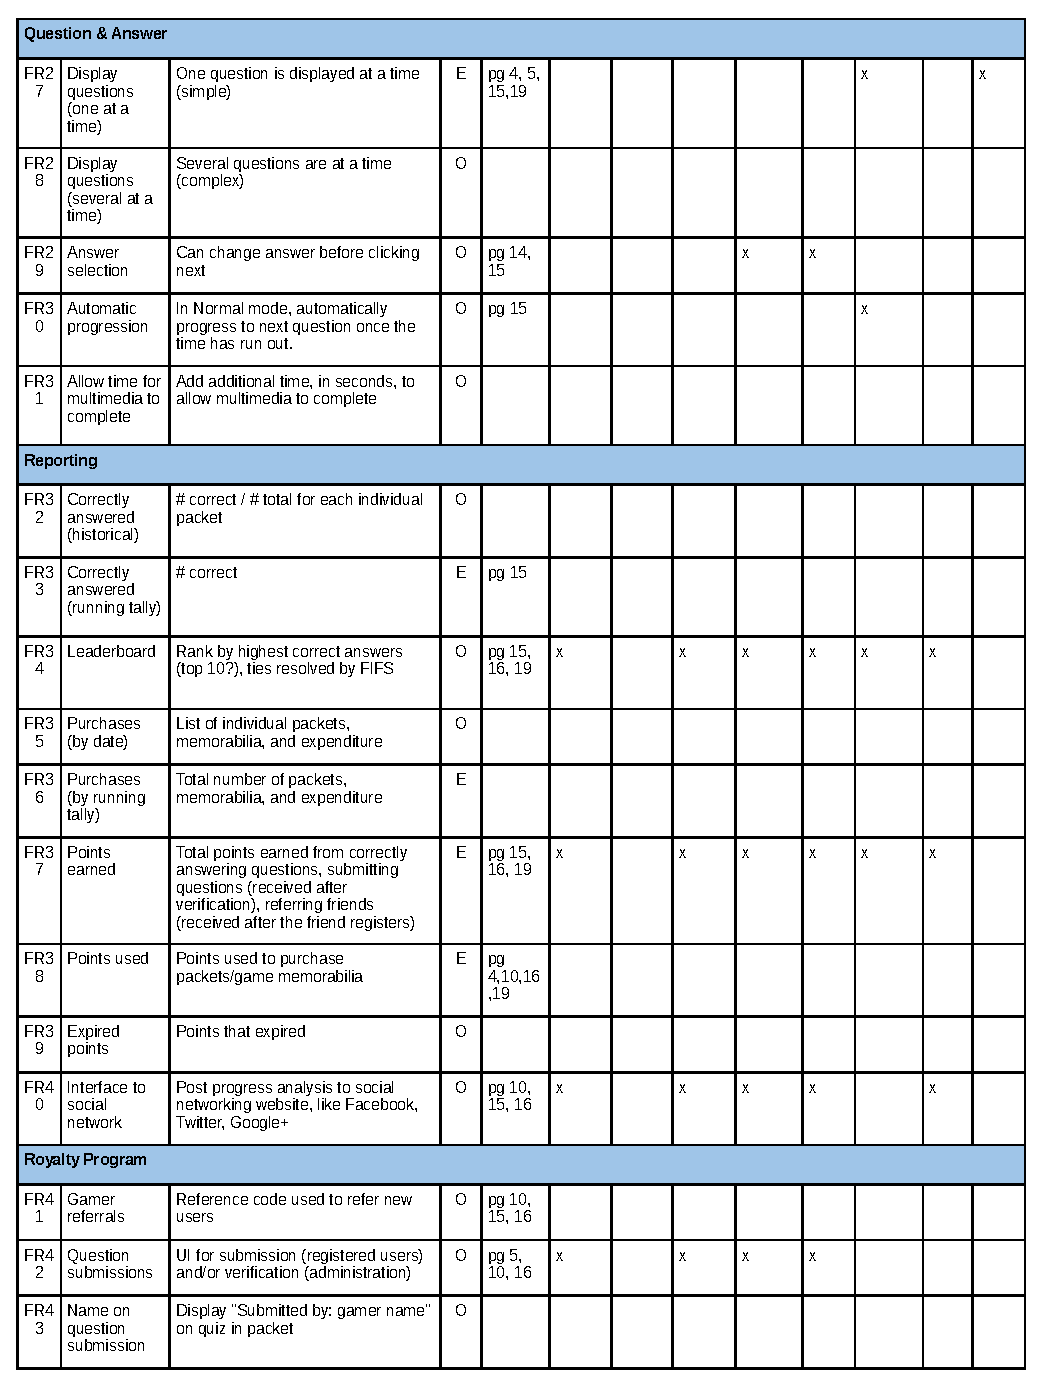
\includegraphics[width=\textwidth]{trace3}
\newpage
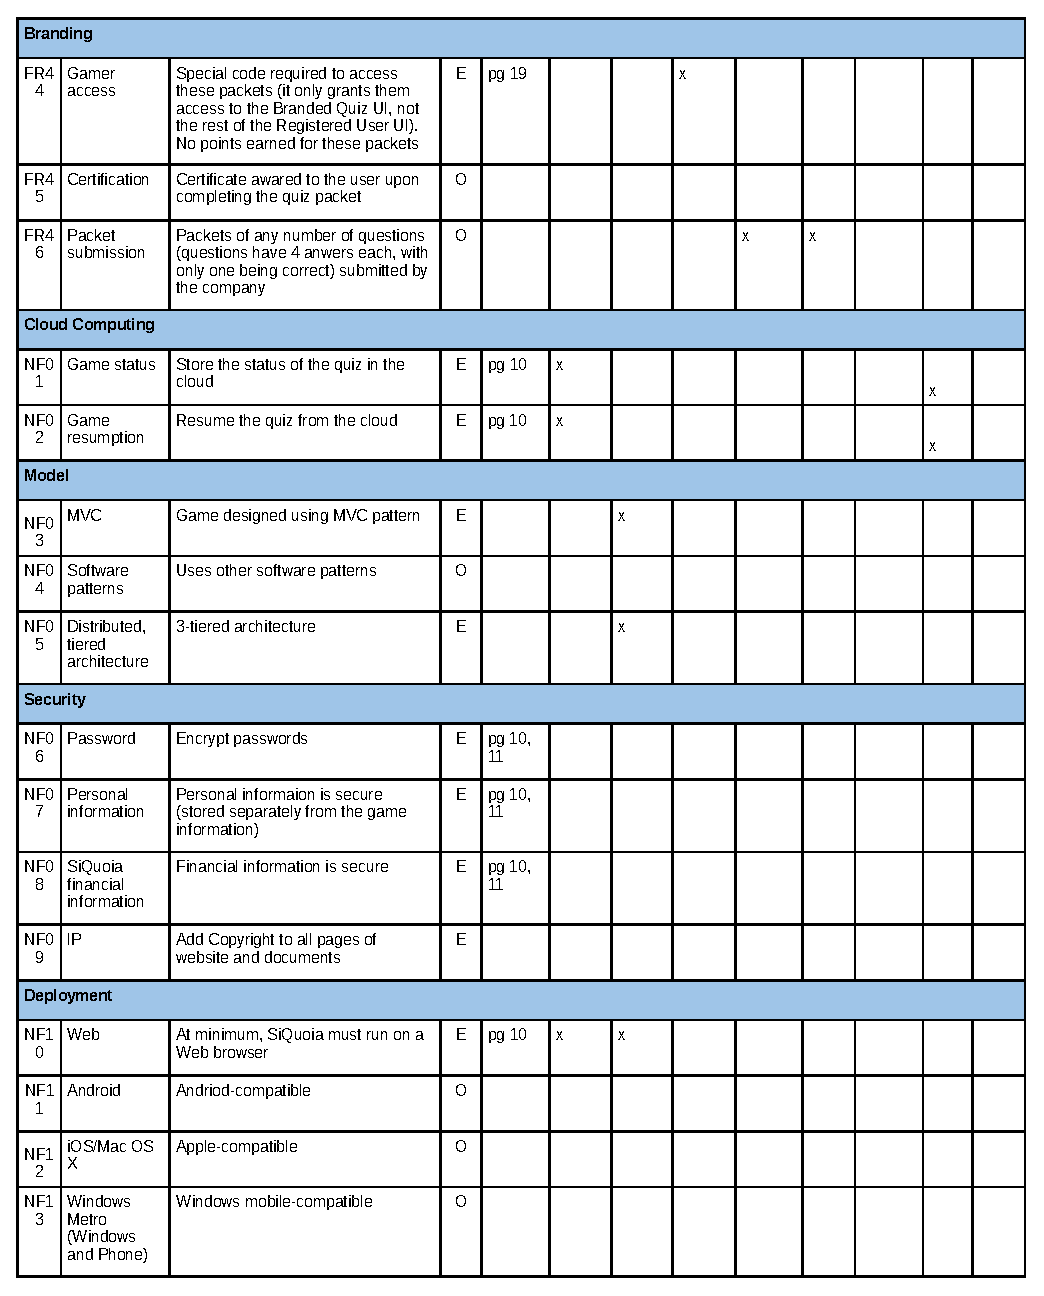
\includegraphics[width=\textwidth]{trace4}
\end{center}

%\vspace*{1in}
%\hspace*{1in}Client signature: \rule{3.2in}{0.25px} \\[-4pt]
%\hspace*{3.2in}{\small Badari S. Eswar}

%\begin{thebibliography}{1}

%\bibitem{IEEEhowto:kopka}
%H.~Kopka and P.~W. Daly, \emph{A Guide to \LaTeX}, 3rd~ed.\hskip 1em plus
%  0.5em minus 0.4em\relax Harlow, England: Addison-Wesley, 1999.

%\end{thebibliography}


\end{document}


